\documentclass[specialist, subf, href, colorlinks=true, 12pt, times, mtpro, final]{disser}
\usepackage [russian] {babel}
\usepackage [utf8] {inputenc}
\usepackage {amsmath}
\usepackage {amsthm}
\usepackage {amssymb}
\usepackage{wrapfig}
\usepackage{enumitem}
\usepackage{amsfonts}
\usepackage{textcomp}
\usepackage{graphicx}
\usepackage{float}
\usepackage{caption}
\usepackage{algorithm}
\usepackage{xcolor}
\usepackage{hyperref}
\usepackage{pdfpages}
\usepackage{dsfont}
\usepackage{upgreek}

\theoremstyle{definition}
\newtheorem{defn}{Определение}[section]
\newtheorem{example}{Пример}[section]
\newtheorem{state}{Утверждение}[section]
\newtheorem{theorem}{Теорема}[section]
\newtheorem{axiom}{Аксиома}[section]

\definecolor{linkcolor}{HTML}{0000FF}
\definecolor{urlcolor}{HTML}{0000FF}
\definecolor{faded}{gray}{0.6}

\def\note{\textcolor{faded}}
\def\rk{\text{rank}}
\def\span{\text{span}}

%---------------------------- defines for bold letters ----------------------------
%                             ( use in mathmode only )
\def\bfrd{\dot{\bfr}}
\def\bfrdd{\ddot{\bfr}}
\def\bfomega{\mathbf{\omega}}
\def\bfrho{\mathbf{\rho}}
\def\bfzero{\mathbf{0}}
%----------------------------------------------------------------------------------

\hypersetup{pdfstartview = FitH, linkcolor = linkcolor, urlcolor = urlcolor, colorlinks = true}

\begin{document}
    
    %\tableofcontents

    \section*{Список вопросов}
    %\note{В этом списке нужно расставить ссылки. Или оглавление сделать. Но так имхо удобнее, т.к. сюда можно по оглавлению возвращаться.}
    \begin{enumerate}
    \item \hyperref[1]{Свободная механическая система. Механическая система со связями. Аксиома освобождения от связей. Силы реакции связей. Уравнения связей. Пространство виртуальных скоростей. Принцип Даламбера – Лагранжа. Уравнения Лагранжа первого рода. Идеальные связи.}
    \item \hyperref[2]{Понятие об интегрируемости связей. Критерий интегрируемости (критерий Фробениуса, без доказательства). Обобщенные координаты системы с интегрируемыми связями. Уравнения дифференциальных связей в обобщенных координатах. Признак неинтегрируемости уравнений связей.}
    \item \hyperref[3]{Принцип Даламбера – Лагранжа в обобщенных координатах. Уравнения Лагранжа второго рода для голономных систем. Обобщенные силы. Работа сил на перемещении вдоль координатной линии. Случай потенциальных сил. Уравнения Лагранжа со множителями в обобщенных координатах.}
    \item \hyperref[4]{Энергия ускорений. Псевдоскорости. Уравнения Аппеля.}
    \item \hyperref[5]{Теоремы об изменении импульса, кинетического момента и кинетической энергии для систем со связями и следствия из них.}
    \item \hyperref[6]{Эквивалентность принципа Даламбера – Лагранжа и уравнений движения свободного твердого тела.}
    \item \hyperref[7]{Уравнения Лагранжа второго рода. Калибровка. Преобразование уравнений при замене координат.}
    \item \hyperref[8]{Первые интегралы уравнений Лагранжа для систем с потенциальными силами:
    интеграл Якоби, интеграл энергии, циклические интегралы. Поле симметрий. Теорема Нетер.}
    \item \hyperref[9]{Понижение порядка уравнений Лагранжа по Раусу. Функция Рауса. Приведенный потенциал. Уравнения Рауса.}
    \item \hyperref[10]{Задача Лагранжа о вращении тяжелого твердого тела вокруг неподвижной точки. Типичное движение оси динамической симметрии. Псевдорегулярная и регулярная прецессии. Способы реализации движений этих типов с заданным углом нутации.}
    \item \hyperref[11]{Равновесия системы уравнений Лагранжа. Соответствующие движения механической системы. Уравнения равновесия. Устойчивость равновесий по Ляпунову. Теорема Лагранжа – Дирихле о достаточном условии устойчивости равновесия.}
    \item \hyperref[12]{Линеаризация уравнений Лагранжа в окрестности состояния равновесия. Существование нормальных координат. Линеаризованные уравнения в нормальных координатах, их интегрирование. Уравнение для собственных чисел. Независимость собственных чисел от выбора координат. Собственные векторы. Выражение матрицы преобразования к нормальным координатам через компоненты собственных векторов.}
    \item \hyperref[13]{Преобразование уравнений Лагранжа в уравнения Гамильтона. Обобщенные импульсы. Явный вид функции Гамильтона для уравнений механики.}
    \item \hyperref[14]{Первые интегралы уравнений Гамильтона. Скобки Пуассона в канонических координатах. Свойства скобок Пуассона, тождество Якоби. Простейшие первые интегралы в случаях независимости функции Гамильтона от времени, наличия циклических координат, отделения переменных.}
    \item \hyperref[15]{Аналог теоремы Нетер для уравнений Гамильтона. Теорема о скобке Пуассона двух первых интегралов. Скобки Пуассона компонент кинетического момента свободной точки.}
    \item \hyperref[16]{Канонические преобразования. Определение, его переформулировка в терминах скобок Пуассона, интерпретация в случае системы с одной степенью свободы.
    Примеры: тождественное, обратное к каноническому, ортогональное преобразование фазовой плоскости, полярные канонические координаты, каноническая перестановка, каноническое изменение масштабов на координатных осях.}
    \item \hyperref[17]{Критерии каноничности преобразования.}
    \item \hyperref[18]{Преобразование уравнений Гамильтона при канонических преобразованиях.}
    \item \hyperref[19]{Производящие функции канонических преобразований (свободного и стандартного). Выражение новой функции Гамильтона через производящие функции в этих случаях.
    Производящие функции для преобразований: тождественного, перехода к полярным каноническим координатам, канонической перестановки, канонического изменения масштабов на координатных осях.}
    \item \hyperref[20]{Уравнения для производящих функций целенаправленных канонических преобразований. Уравнение Гамильтона – Якоби, его полный интеграл. Теорема Якоби. Нахождение полного интеграла в случаях независимости функции Гамильтона от времени, наличия циклических координат, отделения переменных.}
    \item \hyperref[21]{Теорема Лиувилля об интегрировании в квадратурах системы уравнений Гамильтона.}
    \item \hyperref[22]{Канонические отображения в фазовом пространстве в канонических координатах. Каноничность отображения вдоль решений системы уравнений Гамильтона. Сохранение фазового объема при этом отображении. Интегральный инвариант Пуанкаре.}
    \item \hyperref[23]{Интегральный инвариант Пуанкаре – Картана.}
    \item \hyperref[24]{Вариационный принцип Гамильтона в фазовом пространстве системы уравнений Гамильтона.}
    \item \hyperref[25]{Вариационный принцип Гамильтона на конфигурационном многообразии системы уравнений Лагранжа.}
    \item \hyperref[26]{Метод усреднения для систем Гамильтона в стандартной форме. Математический маятник с точкой подвеса, движущейся по эллипсу.}
    \end{enumerate}

    \section{Свободная механическая система. Механическая система со связями. Аксиома освобождения от связей. Силы реакции связей. Уравнения связей. Пространство виртуальных скоростей. Принцип Даламбера – Лагранжа. Уравнения Лагранжа первого рода. Идеальные связи.}
    \label{1}
    \hyperlink {first_lects.1}{Лекции}
    \begin{defn} (\hyperlink{first_lects.1}{Свободная механическая система})\\
    {\it Свободная механическая система} -- система $(m_i, \bfr_i)_{i=1}^N$,\ 
    $\bfr_i = (x_i, y_i, z_i)^T$, движущаяся под действием $\bfF = \left((\bfF_i^T)_{i=1}^N\right)^T
    = \bfF(t,\bfr,\bfrd)$, где $\bfr = \left((\bfr_i^T)_{i=1}^N\right)^T$.
    \end{defn}
    \begin{theorem} (\hyperlink{first_lects.1}{Второй закон Ньютона})\\
    Пусть $\bfr=\bfr(t)$ -- движение $(m_i, \bfr_i)_{i=1}^N$ под действием $\bfF$,
    и $M\bfrdd(t_0) = \bfF|_{\bfr = \bfr(t), \bfrd=\bfrd(t)}|_{t=t_0}$, где
    $M = \text{diag}(m_iE_3)_{i=1}^N$. Тогда $\forall t \in \mathbb{R}$:
    $$M\bfrdd(t) = \bfF|_{\bfr=\bfr(t), \bfrd = \bfrd(t)}.$$
    \end{theorem}
    \begin{defn} (\hyperlink{first_lects.1}{Механическая система со связями})\\
    {\it Механическая система со связями} -- система $(m_i, \bfr_i)_{i=1}^N$, движущаяся под
    действием $\bfF$ с ограничениями на $\bfr$ и $\bfrd$.
    \end{defn}
    \begin{axiom} (\hyperlink{first_lects.1}{Освобождения от связей})\\
    Пусть $\bfr=\bfr(t)$ -- движение $(m_i, \bfr_i)_{i=1}^N$ под действием $\bfF$ со
    связями. Тогда $\exists\  \bfR=\left((\bfR_i^T)_{i=1}^N\right)^T = \bfR(t,\bfr,\bfrd)$,
    что из $M\bfrdd(t_0) = (\bfF + \bfR)|_{\bfr = \bfr(t), \bfrd=\bfrd(t)}|_{t=t_0}$
    следует, что
    $$\forall t \in \mathbb{R}\ \ \ M\bfrdd(t) = (\bfF + \bfR)|_{\bfr = \bfr(t), \bfrd=\bfrd(t)}.$$
    $\bfR$ называется {\bf силами реакции связей}.
    \end{axiom}
    \noindent{\bf Уравнения связей.}\\
    $\{(\bfr^T, \bfrd^T)^T\}$ -- {\it фазовое пространство.}\\
    $\{(t, \bfr^T, \bfrd^T)^T\}$ -- {\it расширенное фазовое пространство.}\\
    Будем считать, что $\forall (t_0, \bfr_0^T, \bfrd_0^T)^T \ \ \exists!$ решение
    $M\bfrdd = \bfF + \bfR$:\\ $\bfr(t_0) = \bfr_0,\ \bfrd(t_0) = \bfrd_0$.\\
    Далее будем рассматривать {\bf связи, линейные по $\bfrd$}.
    $$
    \boxed{
    A\bfrd + \bfa = \bfzero},
    $$
    где $A=A(t,\bfr)\in\text{GL}(\mathbb{R}^k, \mathbb{R}^{3N}),\ \ \bfa=\bfa(t,\bfr)\in\mathbb{R}^k,\ \ \rk(A) = k < 3N$.\\
    \note{(жирным нулем здесь и далее обозначается вектор из нулей)}\\
    \noindent\hyperlink{first_lects.2}{Пример (низ страницы).}\\
    $\bfr\in\mathbb{R}^{3N},\ \ \bfrd, \bfF, \bfR,... \in T_{\bfr}\mathbb{R}^{3N}$,
    $N_{\bfr} = \span\{a_j\}_{j=1}^k$.
    \begin{defn} (\hyperlink{first_lects.3}{Пространство виртуальных скоростей})\\
    $L_{\bfr} = N_{\bfr}^T = \{\bfv\in\mathbb{R}^{3N}:\ A\bfv=\bfzero\} = \text{Ker}(A),$\\
    $\dim N_{\bfr} = k$,\,\, $\dim L_{\bfr} = 3N-k$,\,\,  $T_{\bfr}\mathbb{R}^{3N} = N_{\bfr}\oplus L_{\bfr}$.
    \end{defn}
    \noindent\hyperlink{first_lects.3}{(его свойства тут)}
    \begin{theorem} (\hyperlink{first_lects.3}{Принцип Даламбера-Лагранжа})\\
    $\bfr=\bfr(t)$ -- движение $(m_i, \bfr_i)_{i=1}^N$ под действием $\bfF$ со
    связями $A\bfrd+\bfa=\bfzero$ $\Longleftrightarrow\,\,\,\forall t\in\mathbb{R}:\,$\\
    $\left[ \forall\bfv\in\text{Ker}(A)|_{\bfr=\bfr(t)}:\ \langle M\bfrdd(t)-\bfF-\bfR_L,\bfv\rangle
    |_{\bfr=\bfr(t),\bfrd=\bfrd(t)} = 0,\,\,(A\bfrd+\bfa)|_{\bfr=\bfr(t),\bfrd=\bfrd(t)}=\bfzero \right]$.
    \end{theorem}
    \noindent$\square$ \hyperlink{first_lects.4}{ Доказательство. } $\blacksquare$
    \begin{theorem} (\hyperlink{first_lects.5}{Уравнения Лагранжа первого рода})\\
    $\bfr=\bfr(t)$ -- движение $(m_i, \bfr_i)_{i=1}^N$ под действием $\bfF$ со
    связями $A\bfrd+\bfa=\bfzero$ $\Longleftrightarrow\,\,\,\forall t\in\mathbb{R}:\,$\\
    $\left[ \exists\,\uplambda=\uplambda(t):\ \ M\bfrdd(t)=(\bfF+\bfR_L+A^T\uplambda)|_{\bfr=\bfr(t),\bfrd=\bfrd(t)},\,\,(A\bfrd+\bfa)|_{\bfr=\bfr(t),\bfrd=\bfrd(t)}=\bfzero \right]$.
    \end{theorem}
    \noindent\note{(здесь $\uplambda$ -- вектор)}\\
    \noindent$\square$ \hyperlink{first_lects.6}{ Доказательство. } $\blacksquare$
    \begin{defn}
    Связи называются {\it идеальными}, если $\bfR_L \equiv \bfzero$.
    \end{defn}
    \note{далее будем рассматривать их}
    
    \section{Понятие об интегрируемости связей. Критерий интегрируемости (критерий Фробениуса, без доказательства). Обобщенные координаты системы с интегрируемыми связями. Уравнения дифференциальных связей в обобщенных координатах. Признак неинтегрируемости уравнений связей.}
    \label{2}
	\hyperlink {first_lects.7}{Лекции} \\
	{\bfИнтегрируемые связи:} $A\bfrd+\bfa=\bfzero\,\Leftrightarrow\,\bff=\bfc.$\\
	Система с интегрируемыми связями называется {\it голономной}.
	\begin{theorem} (\hyperlink{first_lects.7}{Критерий Фробениуса, \note{б/д}})\\
	Связь $A\bfrd+\bfa=\bfzero$ -- интегрируемая $\Longleftrightarrow$
	$\forall\,\bfu_1,\bfu_2\in\mathbb{R}^{3N+1}$:\\ $(\langle\bfa_j,\delta\bfr\rangle+a^jdt)(\bfu_1) =
	(\langle\bfa_j,\delta\bfr\rangle+a^jdt)(\bfu_2) = 0, j=\overline{1,k}$ влечет\\
	$d(\langle\bfa_j,\delta\bfr\rangle+a^jdt)(\bfu_1,\bfu_2)=0, j=\overline{1,k}.$
	\end{theorem}

	\section{Принцип Даламбера – Лагранжа в обобщенных координатах. Уравнения Лагранжа второго рода для голономных систем. Обобщенные силы. Работа сил на перемещении вдоль координатной линии. Случай потенциальных сил. Уравнения Лагранжа со множителями в обобщенных координатах.}
	 \label{3}
	\hyperlink {first_lects.14}{Лекции} \\
	
    \section{Энергия ускорений. Псевдоскорости. Уравнения Аппеля.}
     \label{4}
   	\hyperlink {first_lects.19}{Лекции} \\
   	
    \section{Теоремы об изменении импульса, кинетического момента и кинетической энергии для систем со связями и следствия из них.}
    \label{5}
    \hyperlink {first_lects.22}{Лекции} \\
    
    \section{Эквивалентность принципа Даламбера – Лагранжа и уравнений движения свободного твердого тела.}
     \label{6}
    \hyperlink {first_lects.27}{Лекции} \\
    
    \begin{theorem} (Принцип Даламбера-Лагранжа для свободного тв.тела)
    $\bfr = \bfr(t) $ - движение тв.тела $(m_i, \bfr_i)^N_{i=1}$:\\
    $|\bfr_i - \bfr_j| = c_{ij} > 0$, $i < j = 1, ..., N$ под действием 
    $\bfF \Leftrightarrow \forall t \in R$  $\forall \bfv_c$, $\bfomega \in R^3$ $[|\bfr_i - \bfr_j| |_{ \bfr=\bfr(t)=c_{ij}}, i < j = 1,...,N;$  $<M\ddot{\bfr}(t) - \bfF, \bfv>$ $=0$, 
    где $\bfv = ((\bfv_c + ((\bfomega\times\bfrho_i)^T)^N_{i=1})^T]$
    \end{theorem}    
    
    $\square$
    $\dot{\bfr} = \bfv_c + \bfomega\times\bfrho_i \Rightarrow \bfv = ((\bfv_c + ((\bfomega\times\bfrho_i)^T)^N_{i=1})^T$ - параметрическое задание $KerA$. $\blacksquare$\\
    
    \note{\it Формулировка этой херни, которую я нашел в интернете звучит так:\\ Для системы с идеальными связями в любой момент времени сумма элементарных работ активных сил и даламберовых сил инерции равняется нулю. \\Я бы ей не доверял, но, т.к. сам не понимаю формулировку из лекций, думаю, что ляпнуть можно, если докопаются.}
    
     \begin{theorem} (\hyperlink {first_lects.28}{Следствие})
    $\bfr = \bfr(t)$ - движение твердого тела 
    $(m_i, bfr_i)^N_{i=1}$: $|\bfr_i - \bfr_j| = c_{ij} > 0$, $i<j = 1,...,N$ 
    под действием $\bfF$ $\Leftrightarrow$ $\forall t \in R [|\bfr_i - \bfr_j| |_{\bfr=\bfr(t)=c_{ij}}$,
     $i<j=1,...,N$, $m\ddot{\bfr}_c(t)=\sum\limits^N_{i=1} \bfF^{(e)}_i |_{\bfr=\bfr(t), \dot{\bfr}=\dot{\bfr}(t)}$,
      $\frac{d}{dt}K^{(relative)}_c|_{\bfr=\bfr(t), \dot{\bfr}=\dot{\bfr}(t)} = M^{(e)}_c |_{\bfr=\bfr(t), \dot{\bfr}=\dot{\bfr}(t)}]$
      \end{theorem}
     
    
    \section{Уравнения Лагранжа второго рода. Калибровка. Преобразование уравнений при замене координат.}
     \label{7}
    \hyperlink {first_lects.29}{Лекции} \\
    \begin{defn}(Уравнение Лагранжа второго рода
		\begin{center}
 			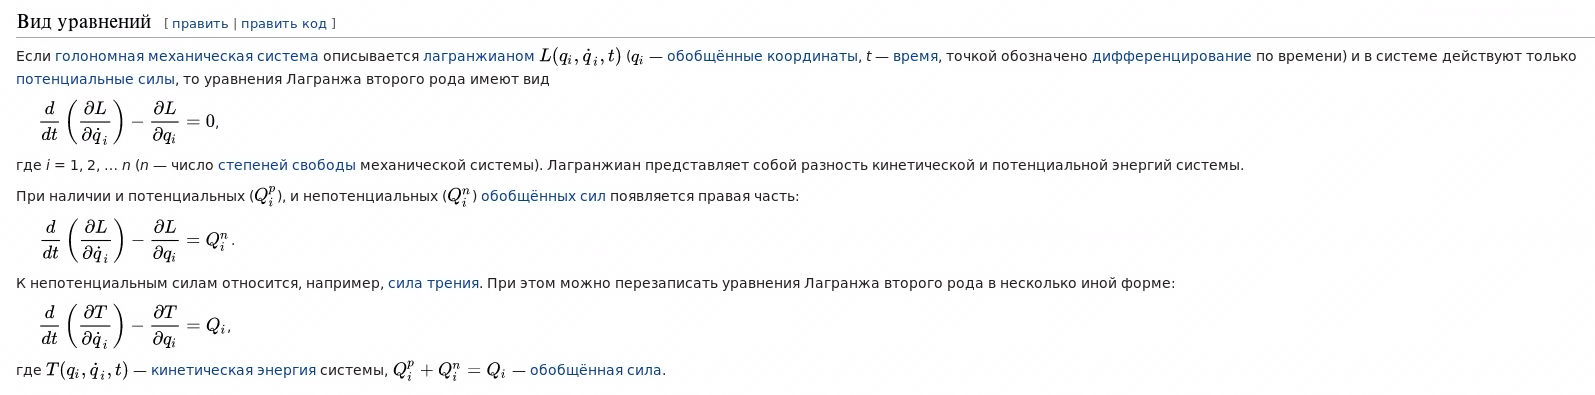
\includegraphics[scale=0.5]{pics/lagranzh}
		\end{center}
	\end{defn}
	
	\hyperlink {first_lects.29}{Вывод, что они имеют второй порядок см.здесь} \\
	
	\textbf{Калибровка} - $L$ и $\widetilde{L}$ дают одинаковые уравнения Лагранжа второго рода:\\
	$\frac{d}{dt}\frac{\partial L}{\partial \dot{\bfq}} - \frac{\partial L}{\partial \bfq} \Leftrightarrow \frac{d}{dt}\frac{\partial \widetilde{L}}{\partial \dot{\bfq}} - \frac{\partial \widetilde{L}}{\partial \bfq}$\\
	Например, $\widetilde{L} = const L$ или $\widetilde{T} = const  T, \widetilde{Q} = const Q$\\
	\note{\it Я понятия не имею, что происходит, но вроде вики говорит калибровка векторного потенциала — наложение дополнительных условий, позволяющих однозначно вычислить векторный потенциал электромагнитного поля для решения тех или иных физических задач.}\\
	
	\hyperlink {first_lects.30}{Пример какой-то калибровки} \\
	
	\begin{theorem}(\hyperlink {first_lects.31}{Теорема о преобразовании при замене к-т})\\
	
	\hyperlink {first_lects.31}{Начальные условия внизу страницы}\\
	
	$\bfx$ - другие локальные к-ты на $M_{const} (t)$\\
	$\frac{d}{dt}[\frac{\partial T}{\partial \dot{\bfx}}|_{\dot{\bfr} = \dot{\bfr}(t, \bfx, \dot{\bfx})}]  -  \frac{\partial T}{\partial \bfx}|_{\dot{\bfr} = \dot{\bfr}(t, \bfx, \dot{\bfx})} = 
	(\frac{d}{dt}[\frac{\partial T}{\partial \dot{\bfq}}|_{\dot{\bfr} = \dot{\bfr}(t, \bfq, \dot{\bfq})}]  -  \frac{\partial T}{\partial \bfq}|_{\dot{\bfr} = \dot{\bfr}(t, \bfq, \dot{\bfq})})|_{\bfq = \bfq(t, \bfx), \dot{\bfq} = \dot{\bfq} (t, \bfx, \dot{\bfx})} \frac{\partial \bfq}{\partial \bfx}$\\
	$\bfX^T =  \bfQ^T |_{\bfq = \bfq(t, \bfx), \dot{\bfq} = \dot{\bfq} (t, \bfx, \dot{\bfx})} \frac{\partial \bfq}{\partial \bfx}$ 
	\end{theorem}
	
	
     
    
    \section{Первые интегралы уравнений Лагранжа для систем с потенциальными силами:    интеграл Якоби, интеграл энергии, циклические интегралы. Поле симметрий. Теорема Нетер.}
     \label{8}
    \hyperlink {lects.1}{Лекции} \\
    
    \section{Понижение порядка уравнений Лагранжа по Раусу. Функция Рауса. Приведенный потенциал. Уравнения Рауса.}
     \label{9}
    \hyperlink {lects.3}{Лекции} \\
    
    \section{Задача Лагранжа о вращении тяжелого твердого тела вокруг неподвижной точки. Типичное движение оси динамической симметрии. Псевдорегулярная и регулярная прецессии. Способы реализации движений этих типов с заданным углом нутации.}
     \label{10}
    \hyperlink {lects.6}{Лекции} \\
    
    \section{Равновесия системы уравнений Лагранжа. Соответствующие движения механической системы. Уравнения равновесия. Устойчивость равновесий по Ляпунову. Теорема Лагранжа – Дирихле о достаточном условии устойчивости равновесия.}
     \label{11}
    \hyperlink {lects.10}{Лекции} \\
    
    \section{Линеаризация уравнений Лагранжа в окрестности состояния равновесия. Существование нормальных координат. Линеаризованные уравнения в нормальных координатах, их интегрирование. Уравнение для собственных чисел. Независимость собственных чисел от выбора координат. Собственные векторы. Выражение матрицы преобразования к нормальным координатам через компоненты собственных векторов.}
     \label{12}
    \hyperlink {lects.11}{Лекции (конец страницы)} \\
    
    \section{Преобразование уравнений Лагранжа в уравнения Гамильтона. Обобщенные импульсы. Явный вид функции Гамильтона для уравнений механики.}
     \label{13}
     \hyperlink {lects.16}{Лекции} \\
    
        
    \section{Первые интегралы уравнений Гамильтона. Скобки Пуассона в канонических координатах. Свойства скобок Пуассона, тождество Якоби. Простейшие первые интегралы в случаях независимости функции Гамильтона от времени, наличия циклических координат, отделения переменных.}
     \label{14}
    \hyperlink {lects.18}{Лекции} \\
    
    \section{Аналог теоремы Нетер для уравнений Гамильтона. Теорема о скобке Пуассона двух первых интегралов. Скобки Пуассона компонент кинетического момента свободной точки.}
     \label{15}
    \hyperlink {lects.18}{Лекции} \\
    
    \section{Канонические преобразования. Определение, его переформулировка в терминах скобок Пуассона, интерпретация в случае системы с одной степенью свободы. Примеры: тождественное, обратное к каноническому, ортогональное преобразование фазовой плоскости, полярные канонические координаты, каноническая перестановка, каноническое изменение масштабов на координатных осях.}
     \label{16}
    \hyperlink {lects.23}{Лекции} \\
    
    \section{Критерии каноничности преобразования.}
     \label{17}
    \hyperlink {lects.25}{Лекции} \\
    
    \section{Преобразование уравнений Гамильтона при канонических преобразованиях.}
     \label{18}
    \hyperlink {lects.27}{Лекции} \\
    
    \section{Производящие функции канонических преобразований (свободного и стандартного). Выражение новой функции Гамильтона через производящие функции в этих случаях. Производящие функции для преобразований: тождественного, перехода к полярным каноническим координатам, канонической перестановки, канонического изменения масштабов на координатных осях.}
     \label{19}
    \hyperlink {lects.28}{Лекции (низ страницы)} \\
    
    \section{Уравнения для производящих функций целенаправленных канонических преобразований. Уравнение Гамильтона – Якоби, его полный интеграл. Теорема Якоби. Нахождение полного интеграла в случаях независимости функции Гамильтона от времени, наличия циклических координат, отделения переменных.}
     \label{20}
    \hyperlink {lects.31}{Лекции} \\
    
    \section{Теорема Лиувилля об интегрировании в квадратурах системы уравнений Гамильтона.}
     \label{21}
    \hyperlink {lects.37}{Лекции} \\
    
    \section{Канонические отображения в фазовом пространстве в канонических координатах. Каноничность отображения вдоль решений системы уравнений Гамильтона. Сохранение фазового объема при этом отображении. Интегральный инвариант Пуанкаре.}
     \label{22}
	\hyperlink {lects.39}{Лекции} \\
    
    \section{Интегральный инвариант Пуанкаре – Картана.}
     \label{23}
    \hyperlink {lects.42}{Лекции} \\
    
    \section{Вариационный принцип Гамильтона в фазовом пространстве системы уравнений Гамильтона.}
     \label{24}
    \hyperlink {lects.44}{Лекции} \\
    
    \section{Вариационный принцип Гамильтона на конфигурационном многообразии системы уравнений Лагранжа.}
     \label{25}
    \hyperlink {lects.45}{Лекции} \\
    
    \section{Метод усреднения для систем Гамильтона в стандартной форме. Математический маятник с точкой подвеса, движущейся по эллипсу.}
     \label{26}
    \hyperlink {lects.47}{Лекции (сразу над формулами)} \\
    
    \includepdf[pages=-, link, linkname = first_lects]{first_lections.pdf}
    \includepdf[pages=-, link, linkname = lects]{Mekhanika_Dist.pdf}
\end{document}
